%----------------------------------------------------------------------------
\chapter{Implementation}
\label{cha:implementation}
%----------------------------------------------------------------------------

At the end of the design step it is clearly visible, what advantages the investigated technologies and tools have. The implementation of the created testing framework represented following the model based testing process phases as earlier.

\begin{figure}[htp]
\centering
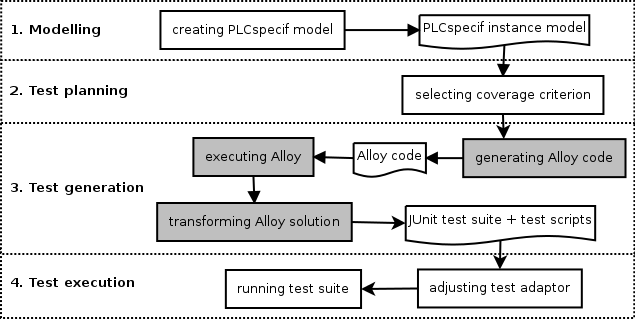
\includegraphics[scale=0.6]{figures/implementation_usage}
\caption{Usage of the test generator framework}
\label{fig:implementation_usage}
\end{figure}

Figure~\ref{fig:implementation_usage} demonstrates the usage of the testing framework. The manual operations are noted with white rectangles, the automatically executed operations are in grey rectangles. Outputs of the operations are represented with document symbols.

The different phases will exemplify the testing of a trivial application, which state machine is showed on Figure~\ref{fig:implementation_trivialsm}. This application has only one method that increases the value of a variable from $0$ to $1$. \texttt{T0} represent the single method the state machine has. Besides that, the state machine has an always satisfiable guard \texttt{G0} , as variable \texttt{output} is initialised to $0$, and an event \texttt{E0} that increases the \texttt{output} variable by $1$. 

\section{Modelling}
\label{sec:implementationmodelling}

First the input model of the testing framework have to be created. This is a PLCspecif instance model created with the default PLCspecif model editor that is generated by the Eclipse Modeling Framework. PLCspecif's generated editor implements all the needed model creation, edition features (UC.1) and model validation as well (UC.2). Concerned components noted on Figure~\ref{fig:designcomponents}, with PLCspecif model, edit framework, model editor and validator.
	
The simplest possible state machine that has all the main UML state machine features showed on Figure~\ref{fig:implementation_model}.
	
\begin{figure}[htp]
\centering
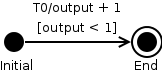
\includegraphics[scale=0.4]{figures/implementation_trivialsm}
\caption{State machine of a trivial SUT}
\label{fig:implementation_trivialsm}
\end{figure}

Constructed models should have some mandatory elements to fully support the test generation process e.g. the JUnit test case generation. The modelled system should have only one state machine module (\texttt{TrivialSM}), where the test model is realised. Each state machine should have a \texttt{VariableDeclaration} named \texttt{output}, one \texttt{CompositeState}, that contains all the \texttt{BasicState}s, from which two has the name \texttt{Initial} and \texttt{End} accordingly.
	
\begin{figure}[htp]
\centering
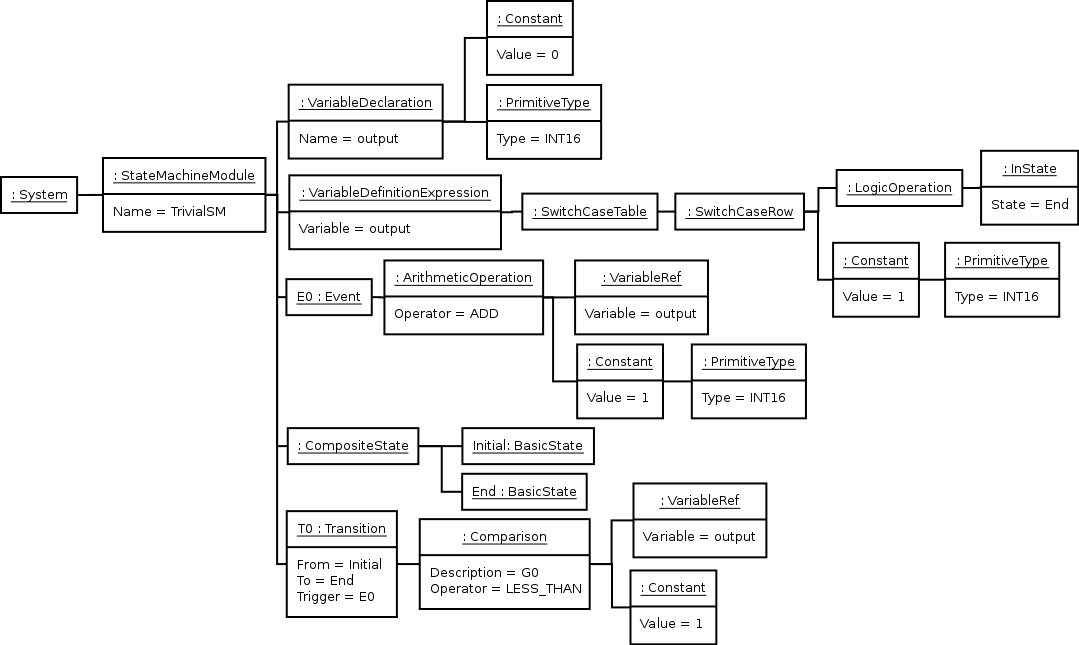
\includegraphics[scale=0.4]{figures/implementation_model}
\caption{Object diagram of a PLCspecif instance model}
\label{fig:implementation_model}
\end{figure}
	
Output assignments is described with a specific \texttt{VariableDefinitionExpression} for \texttt{output} variable. Outputs defined by a switch-case like structure, that has as many \texttt{SwitchCaseRow} as states defined in the state machine. Each row has a condition definition (usually a \texttt{LogicOperation} with a check, that verifies whether the state machine is in a particular state e.g. \texttt{End} state), and a value definition (here represented by a simple \texttt{Constant}). In other words the output of the state machine will be $1$ in the state \texttt{End}.

Transitions can have guard (for example \texttt{G0}) defined on them using \texttt{Comparison} objects. Here \texttt{output} is checked, whether it is less than $1$. Transitions may have attached \texttt{Event}s. For example \texttt{E0} increases the variable \texttt{output} by $1$.

% section modellingimplementation (end)

\section{Test planning}
\label{sec:testplanningimplementation}

At this phase the user can select a test selection criterion (namely full state or transition coverage), which will be used by the test generation. This component is implemented in a separate Eclipse plugin (Test suite generator UI on Figure~\ref{fig:designcomponents}), as the selection is made on the user interface and it is always a good practice to decouple the UI from the business logic.
	
\begin{figure}[htp]
\centering
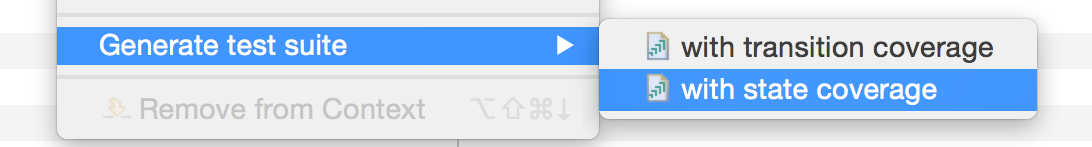
\includegraphics[scale=0.4]{figures/implementation_screenshot}
\caption{Screenshot of the test selection criterion}
\label{fig:implementation_screenshot}
\end{figure}
	
Eclipse SDK exports an extension point \texttt{org.eclipse.ui.popupMenus}, where the context menu of the application can be extended with new actions. So this Eclipse plugin contains two extension, which use this interface to add two new popup menu items.
	
% section testplanningimplementation (end)
	
\section{Test generation}
\label{sec:testgenerationimplementation}
	
When the user selects a test selection criterion on the user interface the test suite generation process will be started automatically. At first the test generation problem will be transformed into Alloy code, that can produce the test cases. The required informations can be extracted from the previously created PLCspecif model, and so the desired Alloy code can be generated automatically. This generation was solved with the model to text transforming capabilities of Acceleo and implemented in a separate Eclipse plugin (Test suite generator on Figure~\ref{fig:designcomponents}).
	
The generated Alloy code has two main parts, the first one consists of statically generated code parts, the other includes highly dynamical, customised structures.
	
Listing~\ref{lst:alloystatic} shows the static parts of the generated Alloy code. Basic structural metamodel of state machines are implemented with signatures (line number  \ref{lst:static1start}-\ref{lst:static1end}). \texttt{System} represents the internal state of the state machine by its state variables. \texttt{State}, \texttt{Transition} objects refer to the traditional EFSM elements. Each state knows its internal state through the \texttt{System} object, and each transitions connects two states.
	
From lines \ref{lst:static2start}-\ref{lst:static2end} metamodel of basic testing object are described. \texttt{Coverage} can refer to a state or transition coverage and so it can be transformed to a test suite. \texttt{Path} is set of method calls within the software, generally more path serve as a \texttt{Coverage}. \texttt{Step} is a method call in the context of software behaviour, but it also connects testing objects to state machine objects.
	
The helper function \texttt{steps} returns a relation containing all steps from a given path. From line number \ref{lst:static3start}-\ref{lst:static3end} are the basic rules of the system. Most of the rules describe the semantics of either the behaviour of state machines or the testing objects. Testing specific model consistency is also verified.

The predicate \texttt{inheritSystem}, is similar to a helper function, but it can only return boolean values if its constraints are satisfiable. This predicate is used to pass along the internal state of the system between the different states.
	
\begin{lstlisting}[label={lst:alloystatic}, caption=Static parts of the generated Alloy code,breaklines=true]
abstract sig System {}(*@\label{lst:static1start}@*)
abstract sig State {system: one System}
abstract sig Transition {from, to: one State}(*@\label{lst:static1end}@*)

sig Coverage { paths: some Path }(*@\label{lst:static2start}@*)
sig Path { firstStep: one Step }
sig Step {
  from, to: one State,
  via: one Transition,
  nextStep: lone Step
} {
  via.from = from
  via.to = to
}(*@\label{lst:static2end}@*)
fun steps (p:Path): set Step { p.firstStep.*nextStep }
fact {(*@\label{lst:static3start}@*)
  // test generation properties
  all p:Path | one c:Coverage | p in c.paths // all path belongs to a coverage
  all s:Step | one p:Path | s in p.firstStep.*nextStep // all steps belongs to a path

  // model consistency
  all p:Path | p.firstStep.from = Initial // all path starts with an Initial state
  all p:Path | one s:Step | s in steps[p] && s.to = End // all path ends with End state
	
  // state machine properties
  all curr:Step, next:curr.nextStep | next.from = curr.to // all steps are continuous
  all sys:System | some s:State | sys = s.system // all system belongs to a state
}(*@\label{lst:static3end}@*)
pred inheritSystem(s1, s2: System) { s1 = s2 }
\end{lstlisting}

Listing~\ref{lst:alloydynamic} shows the dynamic parts of the generated Alloy code. These parts of the Alloy code are generated using the previously created PLCspecif instance model (Figure~\ref{fig:implementation_model}).

Instance models of the \texttt{State} signatures (\texttt{Initial}, \texttt{End}) are instantiated using inheritance. Concrete transitions (\texttt{T0}) are inherited from the \texttt{Transition} object as well. Transitions connected to the initial state have to initialise the internal state variables of the state machine using the dynamically generated \texttt{initSystem} predicate. Guards (\texttt{G0}) and events (\texttt{E0}) connect to these transition objects too.

\begin{lstlisting}[label={lst:alloydynamic}, caption=Dynamic parts of the generated Alloy code,breaklines=true]
one sig Initial, End extends State {}
some sig S extends System {
  output: Int
}
lone sig T0 extends Transition {}{
  from = Initial
  to = End
  initSystem[from.system]
  E0[from.system, to.system]
  G0[from.system]
}
pred E0(s1, s2: System) {
  s2.output = add[s1.output, 1]	
}
pred G0(s: System) {
  s.output < 1
}
pred initSystem(s:System) {
  s.output = 0
}
\end{lstlisting}

Finally Listing~\ref{lst:alloycriteria} show the test criteria formalisation by Alloy predicates. A possible test suite guarantees state coverage if all state present in the union of start and end states of all step in the coverage. Transition coverage is defined in a similar way: a test suite guarantees transition coverage if all transition can be mapped to a step in the coverage.

These criteria are applicable using Alloy's \texttt{run} statements. The constraint solving is executed in a bounded scope, that's why the scope of the search for examples need to be calculated dynamically.

\begin{lstlisting}[label={lst:alloycriteria}, caption=Formalising criteria with Alloy,breaklines=true]
pred state_coverage() {
  all s:State | some p:Path | s in steps[p].from + steps[p].to
}
pred transition_coverage() {
  all t:Transition | some p:Path | t in steps[p].via
}
run state_coverage for 10 but exactly 1 Coverage, 2 System
\end{lstlisting}

The above described generated Alloy code are executed automatically using the Alloy Analyzer API. Operational parameters and other options were fine tuned to get the best possible performance from the integrated SAT solvers. The process of this research will be detailed in Chapter~\ref{cha:measurements}.

When the model is satisfiable and a possible coverage is generated, the solution is parsed into an internal model representation. This internal model is closely related to the testing level and is rather the metamodel of a JUnit test suite.

Similarly to PLCspecif, this internal notation uses a customised Ecore metamodel to describe its behaviour. Instead of starting with a default Ecore model editor, this metamodel is constructed using annotated Java interfaces. Based on them an Ecore model and a generator model is constructed, which will generate the remaining code.

The Alloy solution parser is based on the \textit{Builder} pattern and uses model \textit{Factory} classes from EMF.Edit to create the internal model. After building the test suite model, Acceleo transforms automatically this model to text representation including a complete JUnit test suite (see on Listing~\ref{lst:testsuite}) with pure POJO helper classes.

\begin{lstlisting}[label={lst:testsuite}, caption=Generated JUnit test suite,breaklines=true]
package trivialsm;

import org.junit.Before;
import org.junit.Test;

import junit.framework.TestCase;

public class TrivialSMTest extends TestCase {
	protected TrivialSM trivialsm = null;
	protected TrivialSMTestAdapter adapter = null;
	   
	@Before 
	public void setUp() {
		trivialsm = new TrivialSM();
		adapter = new TrivialSMTestAdapter(trivialsm);
	}
	
	@Test
	public void testPath1() {
		assertEquals(1, adapter.T0());
	}
}
\end{lstlisting}

% section testgenerationimplementation (end)

\section{Test execution}
\label{sec:testexecutionimplementation}

Output of the test generation process consists of three scaffolded helper classes (showed on Figure~\ref{fig:implementation_testhelpers}). They are all generated automatically, derived from the generated test cases and the test model.
	
\begin{description}
	\item[Test suite] is generated as a standard JUnit test fixture (see \texttt{TrivialSMTest} in Listing~\ref{lst:testsuite}). The different test paths are separated into annotated test methods (e.g. \texttt{testPath1}), and a \texttt{setUp} method can be used to initialise the test adapter. Test oracles are generated dynamically in the form of single assertions and inserted into the test methods.
	
	The generated test suite can contain more test paths, which include usually more test cases. A single path starts from the initial state of the SUT and ends in the end state. Set of the paths offer full state or transition coverage within the SUT.
	
	When the user re-generates a test suite for the SUT it can differ from the previously generated test suite, although the generated test suite will have the same structural properties as earlier. This anomaly is, because the execution of the included SAT solver is undetermined.
	\item[Test adapter] scaffolded as a simple POJO class (\texttt{TrivialSMTestAdapter}). This class maps the model transitions to concrete method calls, and also initialisation of the SUT can be done in the adapter's constructor. Method calls wired automatically to concrete SUT's method, using a simple heuristic. If the mapping is not trivial, the adapter's code may not be perfect and needs some adjustment. Here the SUT, named \texttt{TrivialSM} is quite simple, and the adapter does not need any further modification.
	
\begin{figure}[htp]
\centering
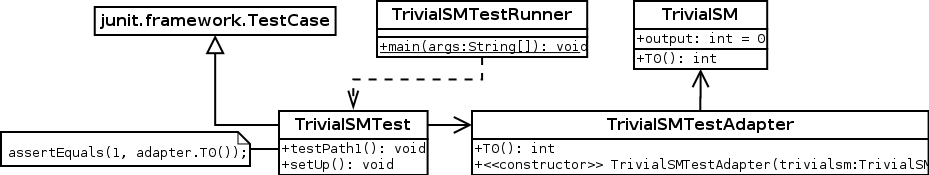
\includegraphics[scale=0.45]{figures/implementation_testhelpers}
\caption{Class diagram of the scaffolded test helpers}
\label{fig:implementation_testhelpers}
\end{figure}

	\item[Test script] is a simple JUnit test runner (\texttt{TrivialSMTestRunner}) that reports the result of the testing. It works like the default JUnit test runner, so it reports out the result of the complete test suite execution (Listing~\ref{lst:successfultestsuite}).

\begin{lstlisting}[label={lst:successfultestsuite}, caption=Successful test suite execution output,breaklines=true]
Finished in 0.005 seconds
1 examples, 0 failures, 0 ignored
\end{lstlisting}
	
	The test reporter tells the difference between the expected and the actual test outcome, moreover if some discrepancy is found it shows the stack trace of the actual exception (Listing~\ref{lst:failedtestsuite}).

\begin{lstlisting}[label={lst:failedtestsuite}, caption=Failed test suite execution output,breaklines=true]
Finished in 0.007 seconds
1 examples, 1 failures, 0 ignored
Failed examples:
testPath1(trivialsm.TrivialSMTest)
junit.framework.AssertionFailedError: expected:<1> but was:<2>
...
\end{lstlisting}
	
\end{description}
	
% section testexecutionimplementation (end)

% chapter implementation (end)